%versi 2 (8-10-2016)
\chapter{Landasan Teori}
\label{chap:teori}


 
Pada bab ini akan dibahas mengenai dasar teori yang digunakan pada penyusunan tugas akhir. Pembahasan pertama mencakup hal-hal yang berkaitan dengan pengertian kewirausahaan dari umum sampai khusus yaitu kewirausahaan menurut GEM. Pembahasan kedua yaitu tentang teori dan aplikasi dari CA (Cellular Automata) khususnya tentang ECA (Entrepreneur Cellular Automata). Pembahasan terakhir tentang hal-hal lain yang mendukung implementasi perangkat lunak seperti bahasa pemrograman java.


\section{Arti Kewirausahaan}
\label{sec:artiwirausaha}

\graphicspath{{images/}}

Wirausaha berasal dari kata wira dan usaha. Wira artinya unggul, mulia, luhur sedangkan usaha berarti kemampuan melakukan usaha atas kekuatan diri sendiri. Jadi wirausaha adalah manusia yang unggul yang memiliki kemampuan membangun usaha sendiri. Kewirausahaan sendiri merupakan kepribadian wirausaha. Wirausaha merupakan orang atau manusia yang memperjuangkan kemajuan terutama pada bidang ekonomi demi masyarakat seperti menciptakan lapangan pekerjaan, membantu memenuhi kebutuhan masyarakat yang semakin meningkat dan berusaha mengurangi ketergantungan dari luar negeri. Istilah kewirausahaan pada umumnya merupakan suatu ilmu yang mempelajari tentang kemampuan seseorang dalam menghadapi tantangan hidup untuk memperoleh peluang dan menghadapi segala risiko yang ada dengan mengandalkan kekuatan diri sendiri tanpa bergantung pada orang lain. \cite{artiwirausaha} 


%Kewirausahaan menurut GEM merupakan proses yang terdiri dari fase-fase berbeda mulai dari niat mendirikan suatu usaha, menjalankan suatu usaha baru atau sudah berdiri dan sampai usaha tersebut berhenti. Proses ini dimulai dengan keterlibatan individu yang berpotensi untuk menjadi wirausaha, yaitu mereka yang percaya bahwa mereka mempunyai kemampuan untuk memulai suatu usaha, individu yang melihat kesempatan untuk berwirausaha dan individu yang tidak takut gagal dalam memulai suatu usaha. \cite{wirausahaGEM}

Kewirausahaan menurut GEM merupakan sebuah proses yang memiliki tahapan-tahapan yang berbeda (Gambar \ref{fig:fasewirausaha}). Tahapan-tahapannya antara lain adalah dimulai dari niat mendirikan usaha, menjalankan usaha dan yang terakhir adalah berhentinya usaha yang dibuat. Tahapan pertama yaitu wirausaha \textit{nascent}. Wirausaha \textit{nascent} ini merupakan tahapan dimana seseorang memulai usahanya yang waktunya kurang dari tiga bulan. Tahapan kedua yaitu wirausaha yang sedang menjalankan usahanya dan sudah bisa menggaji orang lain, waktunya lebih dari tiga bulan tetapi kurang dari tiga tahun. Wirausaha \textit{nascent} dan wirausaha yang sedang menjalankan usahanya masuk ke dalam TEA (Total Early-Stage Entrepreneurial Activity). TEA merupakan persentase populasi antara usia 18 sampai 64 tahun yang berada pada tahap memulai usaha maupun pemilik bisnis yang waktunya kurang dari 42 bulan \cite{wirausahaGEM}. Tahapan terakhir adalah wirausaha mapan (\textit{established entrepreneur}) yaitu seseorang yang sudah menjalankan usahanya lebih dari tiga tahun dan tentunya sudah bisa menggaji orang.\cite{GEM2013}

GEM melakukan penelitiannya berdasarkan pada beberapa premis.Pertama, keadaan ekonomi suatu negara. Jika keadaan ekonomi suatu negara sedang sulit itu artinya dengan adanya wirausaha dapat membantu memperluas lapangan pekerjaan (memotivasi orang untuk menjadi seorang wirausaha juga lebih meningkat), sedangkan jika keadaan ekonomi suatu negara sudah baik keberadaan wirausaha tidak terlalu dibutuhkan (memotivasi orang untuk menjadi seorang wirausaha sudah kurang menarik). Kedua, kemampuan dan motivasi individu untuk memulai sebuah usaha dan pandangan masyarakat tentang wirausaha. Ketiga, pertumbuhan tinggi kewirausahaan dan persaingan antar negara tentang seberapa inovatif usaha tersebut. \cite{GEM2013}
%GEM melakukan penelitiannya dengan didasarkan pada premis-premis berikut. Pertama, kemakmuran sebuah ekonomi sangat tergantung pada sektor kewirausahaan yang dinamis. Sifat dari kegiatan ini dapat beragam karakter dan dampaknya. Kewirausahaan yang didorong oleh kebutuhan khususnya di wilayah yang kurang berkembang atau wilayah yang sedang mengalami penurunan lapangan kerja, dapat membantu ekonomi suatu negara jika memang lapangan pekerjaan terbatas. Di sisi lain, pada wilayah yang lebih berkembang kesempatan wirausaha terjadi lebih akibat dari kemakmuran dan kemampuan inovasi mereka. Kedua, kapasitas kewirausahaan sebuah ekonomi didasarkan pada kemampuan dan motivasi individunya untuk memulai suatu usaha dan dapat diperkuat oleh persepsi positif masyarakat tentang kewirausahaan. Terakhir, pertumbuhan tinggi kewirausahaan adalah kontributor utama untuk penyedia lapangan pekerjaan dan persaingan antar negara bergantung pada usaha yang inovatif.
\begin{figure} [H]
	\centering  
	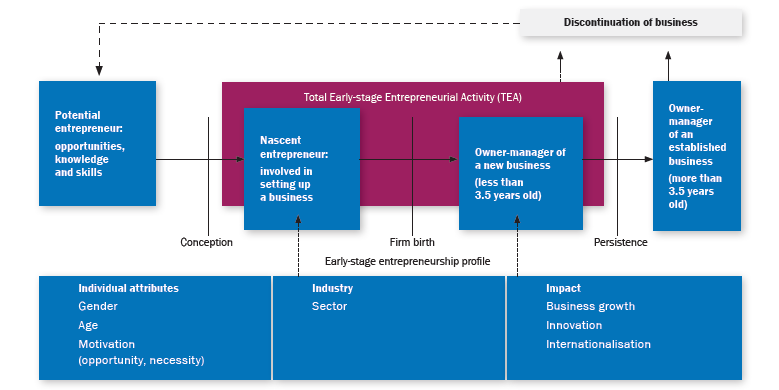
\includegraphics[width=14cm, height=6cm]{GEM2016-wirausaha}  
	\caption[Fase Wirausaha]{Fase Wirausaha} 
	\label{fig:fasewirausaha} 
\end{figure}


GEM mempertimbangkan beberapa atribut atau indikator yang mempengaruhi berlangsungnya kegiatan berwirausaha. Atribut-atributnya yaitu Perceived Opportunities, Perceived Capabilities, Entreprenurial Intention dan Fear of Failure Rate \cite{wirausahaGEM}. Penjelasan beberapa indikator akan dijelaskan pada tabel \ref{tabelindikator}

\begin{table}[H]
\centering
\caption{Tabel Indikator GEM}
\begin{tabular}{|c|p{8cm}|}
\hline
Indikator & Deskripsi\\
\hline
Perceived Opportunities & Persentase penduduk antara usia 18-64 tahun yang melihat peluang baik untuk memulai usaha. \\
\hline
Perceived Capabilities & Persentase penduduk antara usia 18-64 tahun yang percaya bahwa mereka mempunyai kemampuan untuk memulai suatu usaha. \\
\hline
Entreprenurial Intention & Persentase penduduk antara usia 18-64 tahun (selain orang yang berwirausaha) yang bertekad untuk mendirikan usaha dalam waktu tiga tahun kedepan.\\
\hline
Fear of Failure Rate & Persentase penduduk antara usia 18-64 tahun dapat melihat peluang baik yang mengindikasikan bahwa takut akan gagal akan menjauhkan mereka dari mendirikan usaha. \\
\hline
Role Model & Persentase penduduk antara usia 18-64 tahun yang memulai bisnis pada dua tahun terakhir.\\
\hline
\end{tabular}
\label{tabelindikator}
\end{table}



Indikator-indikator menurut GEM yang mempengaruhi perkembangan kewirausahaan di Indonesia yaitu Perceived Capabilities, Role Model, Perceived Opportunity dan Fear of Failure. Berikut data pendidikan dan wilayah Indonesia dari GEM tentang Perceived Capabilities yang diambil pada tahun 2015 \cite{dataGEM}.


\begin{figure} [H]
	\centering  
	\includegraphics[width=14cm, height=7cm]{PCPendidikan} 
	\caption[Komposisi perceived capabilities untuk tingkat pendidikan yang berbeda]{Komposisi perceived capabilities untuk tingkat pendidikan yang berbeda} 
	\label{fig:PCPendidikan} 
\end{figure}

Dapat dilihat pada gambar \ref{fig:PCPendidikan} dijelaskan bahwa individu yang memiliki kemampuan berwirausaha tertinggi yaitu pada individu yang berpendidikan sekolah menengah ke atas (SMA). Pria mempunyai peluang yang lebih unggul (58.5\%) daripada wanita (55.4\%). Peluang yang paling rendah untuk menjadi wirausaha yaitu pada individu yang berpendidikan sampai S-3 yaitu 0.0\% untuk wanita dan 0.1\% untuk pria. 

\begin{figure} [H]
	\centering  
	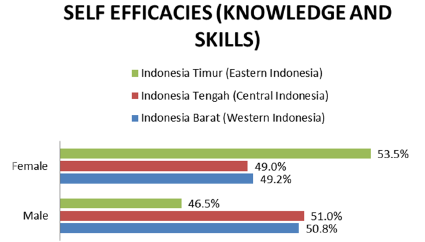
\includegraphics[width=11cm, height=6cm]{PCRegion} 
	\caption[Komposisi perceived capabilities untuk wilayah Indonesia]{Komposisi perceived capabilities untuk wilayah Indonesia} 
	\label{fig:PCRegion} 
\end{figure}

Dapat dilihat pada gambar \ref{fig:PCRegion} dijelaskan bahwa individu yang memiliki kemampuan berwirausaha tertinggi yaitu pada wanita yang berada pada wilayah Indonesia Timur sebesar 53.5\% sedangkan pria yang berpeluang tinggi untuk menjadi wirausaha berada pada wilayah Indonesia Tengah sebesar 51.0\%. Individu yang memiliki kemampuan berwirausaha terendah yaitu untuk wanita berada pada wilayah Indonesia Tengah sebesar 49.0\% dan untuk pria berada pada wilayah Indonesia Timur sebesar 46.5\%. Data kedua yaitu data Role Model tentang perbedaan tingkat wirausaha antara perempuan dan laki-laki serta yang kedua adalah data pendidikan.

\begin{figure} [H]
	\centering  
	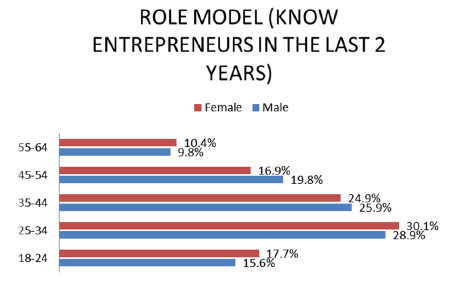
\includegraphics[width=12cm, height=7cm]{RMfemalemale} 
	\caption[Komposisi role model untuk wanita dan pria]{Komposisi role model untuk wanita dan pria} 
	\label{fig:RMfemalemale} 
\end{figure}


Pada gambar \ref{fig:RMfemalemale} dijelaskan individu yang memulai bisnis dalam 2 tahun terakhir. Peluang individu yang memulai bisnis dalam 2 tahun terakhir tertinggi yaitu pada wanita usia 25 sampai 34 tahun sebesar 30.1\% sedangkan pria sebesar 28.9\%. Peluang terendah yaitu pada wanita usia 55 sampai 64 tahun sebesar 10.4\% sedangkan pria sebesar 9.8\%.


\begin{figure} [H]
	\centering  
	\includegraphics[width=13cm, height=7cm]{RMpendidikan} 
	\caption[Komposisi role model untuk tingkat pendidikan yang berbeda]{Komposisi role model untuk tingkat pendidikan yang berbeda} 
	\label{fig:RMpendidikan} 
\end{figure}  


Pada gambar \ref{fig:RMpendidikan} dijelaskan individu yang memulai bisnis dalam 2 tahun terakhir. Peluang individu yang memulai bisnis dalam 2 tahun terakhir tertinggi pada individu yang mempunyai tingkat pendidikan sekolah menengah ke atas (SMA). Pria memperoleh persentase sebesar 58.3\% dan wanita sebesar 54.4\%. Individu yang mempunyai peluang terendah yaitu individu yang berpendidikan S-3. Pria memperoleh persentase sebesar 0.1\% dan wanita memperoleh persentase sebesar 0.0\%. Data ketiga yaitu data Perceived Opportunities tentang perbedaan tingkat wirausaha antara perempuan dan laki-laki serta yang kedua adalah data pendidikan.

\begin{figure} [H]
	\centering  
	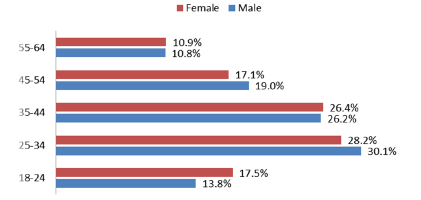
\includegraphics[width=12cm, height=6cm]{POfemalemale} 
	\caption[Komposisi role model untuk wanita dan pria]{Komposisi role model untuk wanita dan pria} 
	\label{fig:POfemalemale} 
\end{figure} 

Pada gambar \ref{fig:POfemalemale} dijelaskan kemampuan individu antara pria dan wanita dalam melihat peluang berwirausaha. Peluang tertinggi yaitu pada pria berusia 25 sampai 34 tahun yang memiliki persentase sebesar 30.1\% dan wanita sebesar 28.2\%. Peluang terendah yaitu pada pria berusia 55 sampai 64 tahun sebesar 10.8\% dan wanita sebesar 10.9\%. 

\begin{figure} [H]
	\centering  
	\includegraphics[width=14cm, height=6cm]{POpendidikan} 
	\caption[Komposisi perceived opportunities untuk tingkat pendidikan yang berbeda]{Komposisi perceived opportunities untuk tingkat pendidikan yang berbeda} 
	\label{fig:POpendidikan} 
\end{figure}  

Gambar \ref{fig:POpendidikan} menjelaskan kemampuan individu dalam melihat peluang. Kemampuan melihat peluang berwirausaha tertinggi yaitu pada individu yang berpendidikan sekolah menengah ke atas (SMA). Persentase pria sebesar 59.3\% dan wanita sebesar 56.7\%. Kemampuan melihat peluang berwirausaha terendah yaitu pada individu yang berpendidikan S-3. Persentase pria sebesar 0.2\% dan wanita sebesar 0.0\%. Data keempat yaitu data Fear of Failure tentang perbedaan tingkat wirausaha antara perempuan dan laki-laki.

\begin{figure} [H]
	\centering  
	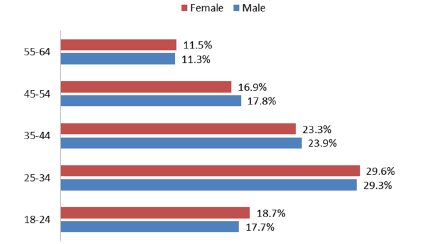
\includegraphics[width=13cm, height=6cm]{FOFfemalemale} 
	\caption[Komposisi fear of failure untuk wanita dan pria]{Komposisi fear of failure untuk wanita dan pria} 
	\label{fig:FOF} 
\end{figure}  

Gambar \ref{fig:FOF} menjelaskan perbedaan Fear of Failure antara pria dan wanita. Persentase Fear of Failure yang tertinggi yaitu pada wanita berusia 25 sampai 34 tahun sebesar 29.6\% dan pria sebesar 29.3\%. Persentase Fear of Failure terendah yaitu pada wanita usia 55 sampai 64 tahun sebesar 11.5\% dan pria sebesar 11.3\%. 

\section{Cellular Automata}
\label{sec:cellularautomata}

Cellular Automata (CA) diperkenalkan pertama kali oleh Ulam dan von Neumann pada tahun 1940. Cellular Automata sendiri merupakan model matematis untuk sistem dimana banyak komponen sederhana bertindak bersama untuk menghasilkan pola perilaku yang rumit \cite{referensiCA2}. Sebuah CA terdiri atas sekumpulan sel, tersusun dalam larik-larik (\textit{grid}). Setiap sel mempunyai satu dari sejumlah \textit{state} (kondisi) yang mungkin. \textit{State} dapat berubah sesuai dengan aturan tertentu. Perubahan \textit{state} dari sebuah sel dipengaruhi oleh \textit{state} dari sel-sel di sekitarnya atau disebut dengan sel tetangga.

\subsection{Karakteristik CA}
\begin{enumerate}
	\item Dimensi pada CA
		\begin{enumerate}
			\item CA Satu Dimensi
			
				\begin{figure} [H]
					\centering  
					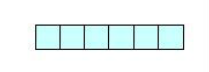
\includegraphics[width=4cm, height=2cm]{CA1D} 
					\caption[CA 1 Dimensi]{CA 1 Dimensi} 
					\label{fig:CA1D} 
				\end{figure}
			
			Cellular Automata satu dimensi adalah cellular automata yang ruang selnya berupa array satu dimensi, sehingga masing-masing sel hanya memiliki dua tetangga yang tepat bersebelahan, kecuali sel paling pinggir yang hanya mempunyai satu tetangga. CA satu dimensi biasanya memakai aturan yang diusulkan oleh Wolfram. Sebagai contoh berikut aturan no. 30 diberikan pada gambar \ref{fig:wolfram}
			
			
			\begin{figure} [H]
					\centering  
					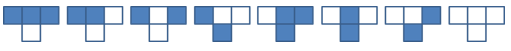
\includegraphics[width=10cm, height=2cm]{wolfram} 
					\caption[Aturan 30 dari Wolfram]{Aturan 30 dari Wolfram} 
					\label{fig:wolfram} 
				\end{figure}
				
				Cara membaca aturan tersebut adalah pada baris pertama terdapat 3 sel pada suatu saat (iterasi) tertentu, sel yang ditinjau adalah sel yang berada di tengah. Tetangga dari sel tersebut yaitu tetangga kiri dan kanan. Baris kedua menunjukkan keadaan sel pada \textit{state} berikutnya. Sebagai contoh pada gambar paling kiri, sel pada bagian tengah (gelap) mempunyai tetangga kiri gelap dan tetangga kanan gelap maka iterasi berikutnya \textit{state} sel tersebut berubah menjadi putih.
				
				Sebagai ilustrasi, pada gambar \ref{fig:penerapanwolfram} diberikan contoh penerapan aturan 30 dari Wolfram yang dimulai dari kondisi awal (t=0) dengan sel gelap yang berada di tengah hingga t=9. \cite{ECA}
				
				\begin{figure} [H]
					\centering  
					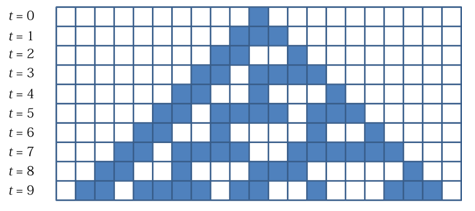
\includegraphics[width=10cm, height=6cm]{penerapanwolfram} 
					\caption[Ilustrasi penerapan aturan 30 dari Wolfram]{Ilustrasi penerapan aturan 30 dari Wolfram} 
					\label{fig:penerapanwolfram} 
				\end{figure}
				
			\item CA Dua Dimensi
			
			\begin{figure} [H]
					\centering  
					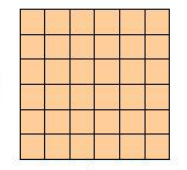
\includegraphics[width=4cm, height=2cm]{CA2D} 
					\caption[CA 2 Dimensi]{CA 2 Dimensi} 
					\label{fig:CA2D} 
				\end{figure}
			
			Cellular Automata dua dimensi adalah cellular automata yang ruang selnya biasanya berupa matriks, sehingga masing-masing sel memiliki lebih dari dua tetangga. CA dua dimensi yang sangat terkenal adalah Conway's \textit{Game of Life}. Setiap sel pada CA menggambarkan suatu individu yang dapat berada pada \textit{state} hidup atau mati. Sel hidup dapat berubah menjadi mati dan sel mati dapat berubah menjadi sel hidup. Aturan dasar Conway's diberikan pada gambar \ref{fig:conway}
			
			
			\begin{figure} [H]
					\centering  
					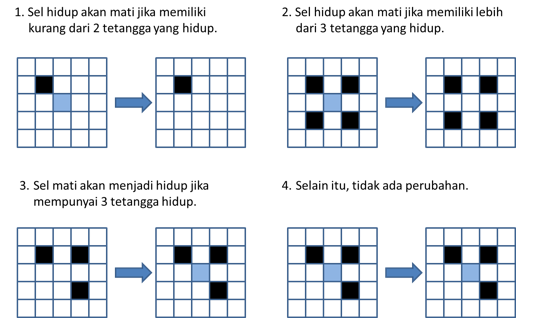
\includegraphics[width=12cm, height=8cm]{conway} 
					\caption[Aturan Dasar Conway's Game of Life]{Aturan Dasar Conway's Game of Life} 
					\label{fig:conway} 
				\end{figure}
			
			Berikut ilustrasi Conway yang menggambarkan perubahan yang terjadi pada sekumpulan sel mulai dari kondisi awal (t=0) sampai dengan kondisi akhir (t=3) yang dilakukan secara iteratif. Banyaknya sel hidup pada kondisi awal berkurang sedikit demi sedikit sampai pada kondisi akhir tidak ada lagi sel hidup. \cite{ECA}
			
			
			\begin{figure} [H]
					\centering  
					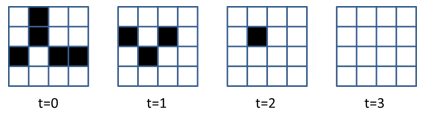
\includegraphics[width=10cm, height=3cm]{contohconway} 
					\caption[Ilustrasi Conway's Game of Life]{Ilustrasi Conway's Game of Life} 
					\label{fig:contohconway} 
				\end{figure}
			
		
	\item Aplikasi CA
		
		\begin{enumerate}
			\item Bidang Transportasi
			
			CA banyak digunakan untuk memodelkan lalu lintas, dengan tujuan utama biasanya adalah untuk mempelajari beban dari jalan-jalan di area tertentu. Contoh aplikasi CA dibidang transportasi ini adalah simulasi pengaturan lampu lalu lintas. Model dalam penelitian ini menggunakan CA 1 dimensi. Pada pergerakan  atau perpindahan lajur kendaraan, terdapat beberapa aturan yaitu : 

	\begin{figure} [H]
		\centering  
		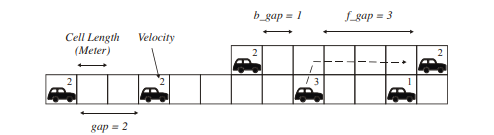
\includegraphics[width=12cm, height=4cm]{aplikasi1} 
		\caption[Ilustrasi dua jalur]{Ilustrasi dua jalur} 
		\label{fig:aplikasiCA1} 
	\end{figure}
				\begin{enumerate}
				\item Kendaraan di depannya terlalu dekat (kecepatan >   \textit{gap}).
				\item Jalur di sebelahnya kosong.
				\item f\_gap $\geq$ kecepatan.
				\item b\_gap $\geq$ kecepatan\_maksimum.
				\item Peluang untuk pindah terpenuhi (rand() $\leq$ peluang\_pindah). \cite{referensiCA3}
			
			\end{enumerate}
			
			
			\item Bidang Kesehatan
			
			Pada bidang kesehatan, CA juga sering digunakan untuk pemodelan penyebaran penyakit. Biasanya masalah penyebaran penyakit dimodelkan dengan CA dua dimensi dan menggunakan aturan Game of Life dari Conway. Contoh aplikasi yang diterapkan di dunia nyata yaitu simulasi infeksi virus influenza A menggunakan cellular automaton. Pada penelitian ini cellular automata yang digunakan adalah CA dua dimensi. CA yang dibangun akan memodelkan CA yang memiliki \textit{lattice} berbentuk segienam sebagai penyederhanaan dari bentuk bola ke dalam dua dimensi, hal ini dikarenakan sel tubuh manusia berbentuk seperti bola. Pada penelitian ini digunakan batasan secara \textit{periodic}, dengan asumsi sel yang berseberangan sebenarnya bersebelahan pada kondisi aslinya karena masing-masing virus hanya dapat menginfeksi jaringan tubuh tertentu saja. \cite{referensiCA1}
			
			\item Bidang Lingkungan / Ekologi
			
			CA juga dapat digunakan untuk pemodelan pada bidang lingkungan. Contoh penerapan cellular automata pada bidang lingkungan adalah simulasi dan pemodelan perubahan penggunaan lahan. Penelitian ini menggunakan algoritma DINAMICA, algoritma ini merupakan algoritma cellular automata hibrida yang mendukung pemodelan statistik untuk menemukan area yang berpotensi mengalami perubahan berdasarkan faktor pemicu yang telah ditentukan. Algoritma DINAMICA ini memerlukan beberapa parameter berupa :
			\begin{enumerate}
				\item Variabel statis dan dinamis
				
				Variabel statis yang dimaksud adalah data penggunaan lahan multiwaktu yang dijadikan referensi fakta dalam pemodelan. Variabel dinamis adalah jarak setiap piksel dari penggunaan lahan perkotaan ke lahan bukan perkotaan terdekat.
				\item Matriks transisi
				
				Matriks transisi diperoleh dari persilangan tabulasi penggunaan lahan. Hasil dari persilangan ini adalah tingkat perubahan penggunaan lahan dalam satuan persen yang memperlihatkan banyaknya piksel yang terkonversi dari penggunaan lahan yang satu ke penggunaan lahan yang lain (bukan perkotaan ke perkotaan).
				\item Probabilitas Transisi Spasial
				
				Probabilitas Transisi Spasial adalah kemungkinan perubahan dari penggunaan lahan bukan perkotaan ke penggunaan lahan perkotaan.
				\item Fungsi Transisi
				
				Fungsi kalkulasi melakukan kalkulasi pemilihan piksel yang akan berubah dalam dua prosedur yaitu fungsi perluasan yang diaplikasikan pada \textit{path dependent} dan fungsi tapak yang diaplikasikan pada kejadian spontan (random). \cite{referensiCA4}
			\end{enumerate}
			
			\item Bidang Sains
			
			Pada bidang sains, khususnya fisika CA dapat digunakan untuk memodelkan pergerakan partikel dan juga permasalahan lainnya terkait dengan fisika kuantum. Pada bidang biologi, CA digunakan untuk memodelkan sel biologis.
		\end{enumerate}
		
\end{enumerate}

\section{Entrepreneurial Cellular Automata}
\label{sec:ECA}
Entrepreneurial Cellular Automata merupakan pengembangan model dari Cellular Automata yang digunakan untuk mensimulasikan pertumbuhan kewirausahaan di Indonesia. Dalam kasus Entrepreneurial Cellular Automata (ECA), sel akan merepresentasikan wirausahawan dan ketetanggaannya akan merepresentasikan hubungan antar wirausahawan. Setiap wirausahawan mempunyai dua sifat atribut yaitu statis (nilainya tidak berubah) dan dinamis (nilainya dapat berubah). Contoh atribut statis adalah bidang usaha, kategori usaha, lokasi geografis dan jenis kelamin. Contoh atribut dinamis adalah usia, level wirausaha dan usia usaha.  

Perubahan atribut dinamis dari waktu ke waktu didefinisikan dengan fungsi transisi. Fungsi transisi terdiri dari beberapa aturan. Atribut penting dalam kewirausahaan yaitu level wirausaha karena atribut ini digunakan untuk menentukan perkembangan dari kewirausahaan. Cara menentukan seorang wirausaha akan meneruskan usahanya diketahui dari sebuah angka yang disebut \textit{Continuity Index} (\textit{CIdx}). \textit{CIdx} dari seorang wirausaha tidak hanya dipengaruhi oleh faktor dari dalam tetapi juga dipengaruhi oleh faktor dari luar. Faktor luar dipengaruhi oleh tetangga-tetangganya seperti kebijakan pemerintah, kondisi perekonomian dunia, dsb. Seorang wirausahawan akan meneruskan usahanya jika \textit{CIdx}-nya memenuhi nilai ambang tertentu.

Atribut dari seorang wirausahawan dapat berubah dari waktu ke waktu, hal ini menyebabkan ketetanggaan juga dapat berubah dari waktu ke waktu. Sebagai contoh, diasumsikan terdapat wirausahawan $e1$ dan $e2$ bertetanggaan pada waktu $t$, jika $e1$ berubah keadaannya pada $t+1$ maka $e1$ dan $e2$ tidak lagi bertetanggaan pada saat $t+1$.

\subsection{Definisi ECA}
Diberikan \textit{p} himpunan nilai atribut: $A_{1}, ..., A_{p}$ dan sebuah indikator $Pub$ = ${p_{1}, ..., p_{m}}$, sebuah ECA $M$ adalah sebuah tupel
\begin{displaymath}
	M = (E, \alpha, N, \omega, \rho, \delta, \sigma)
\end{displaymath}
dimana :
\begin{itemize}
	\item $E = {e_{1}, ..., e_{n}}$ adalah himpunan berhingga wirausahaan,
	\item $\alpha = {\alpha_{1}, ..., \alpha_{p}}$ adalah himpunan berhingga atribut dimana setiap $\alpha_{i}$ didefinisikan sebagai $\alpha_{i} : E \rightarrow A_{i}$,
	\item $N = {N_{1}, ..., N_{k}}$ adalah himpunan berhingga ketetanggaan dimana setiap $N_{i}$ didefinisikan sebagai $N_{i}:E \times E \rightarrow \Re$,
	\item $\omega = {\omega_{1}, ..., \omega_{k}}$ adalah himpunan fungsi bobot atau nilai ketetanggaan dimana $\omega_{i} : N_{i} \rightarrow \Re$ memetakan setiap fungsi ketetanggaan ke sebuah bilangan riil,
	\item $\rho = {\rho_{1}, ..., \rho_{p}}$ adalah himpunan indikator publik dimana setiap $\rho_{i}$ didefinisikan sebagai $\rho_{i} : p_{i} \rightarrow \Re$,
	\item $\delta : \beta \rightarrow \beta$ adalah fungsi transisi state, dan
	\item $\sigma : N \rightarrow N$ adalah sebuah fungsi transformasi ketetanggaan.
\end{itemize}


Berdasarkan model kewirausahaan terdapat empat tingkatan wirausaha yaitu \textit{potential}, \textit{nascent}, \textit{new business manager} dan \textit{manager of established business}. Akan ditambahkan pula tingkatan wirausaha yang menyatakan wirausahawan di atas umur 64 tahun yaitu \textit{retired}. Pada gambar \ref{fig:tingkatwirausaha} akan ditunjukkan secara lebih lanjut, \textit{new\_bm} dan \textit{est\_bm} dinyatakan sebagai \textit{new business manager} dan \textit{manager of established business}.


	\begin{figure} [H]
		\centering  
		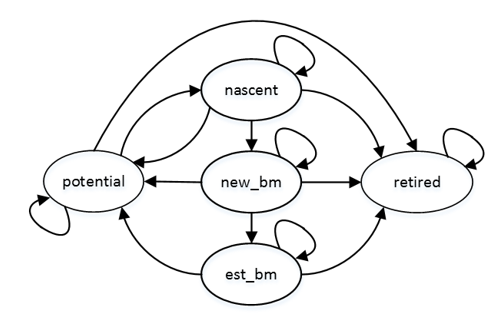
\includegraphics[width=9cm, height=5cm]{tingkatwirausaha} 
		\caption[Diagram Transisi Level Wirausaha]{Diagram Transisi Level Wirausaha} 
		\label{fig:tingkatwirausaha} 
	\end{figure}


Perubahan dari satu level ke level yang lain berdasarkan pada sebuah nilai yang dinamakan Continuity Index, selain usia usaha dan usia individu. Pada tabel \ref{tabelLW} akan dijelaskan mengenai transisi level dengan menggunakan lambang-lambang \textit{CIdx, bl, a ,b} dan \textit{th} untuk menyatakan \textit{Continuity Index, level} , usia individu, usia usaha dan nilai ambang. Nilai ambang ini digunakan sebagai syarat minimal yang harus dipenuhi wirausahawan untuk dapat meneruskan usahanya. Sebagai satu waktu digunakan bulan.

\begin{table}[H]
\centering
\caption{Transisi Level Wirausaha}
\begin{tabular}{|c|c|}
\hline
Waktu sekarang & Waktu berikutnya \\
\hline
\textit{bl} = potential, $ \textit{CIdx} < \textit{th}, \textit{a} < 64 \times 12$ & \textit{bl} = potential \\
\hline
\textit{bl} = potential, $\textit{CIdx} \geq \textit{th}, \textit{a} < 64 \times 12$ & \textit{bl} = nascent \\
\hline
\textit{bl} = potential, $\textit{a} \geq 64 \times 12$ & \textit{bl} = retired \\
\hline
\textit{bl} = nascent, $\textit{CIdx} < \textit{th}, \textit{a} <64 \times 12$ & \textit{bl} = potential \\
\hline
\textit{bl} = nascent, $\textit{CIdx} \geq \textit{th}, \textit{b} < 3$ & \textit{bl} = nascent \\
\hline
\textit{bl} = nascent, $\textit{a} \geq 64 \times 12$ & \textit{bl} = retired \\
\hline
\textit{bl} = new\_bm, $\textit{CIdx} < \textit{th}, \textit{a} < 64 \times 12$ & \textit{bl} = potential \\
\hline
\textit{bl} = new\_bm, $\textit{CIdx} \geq \textit{th}, \textit{b} < 42$ & \textit{bl} = potential \\
\hline
\textit{bl} = new\_bm, $\textit{a} \geq 64 \times 12$ & \textit{bl} = retired \\
\hline
\textit{bl} = est\_bm, $\textit{CIdx} < \textit{th}, \textit{a} < 64 \times 12$ & \textit{bl} = potential \\
\hline
\textit{bl} = est\_bm, $\textit{CIdx} \geq \textit{th}, \textit{a} < 64 \times 12$ & \textit{bl} = est\_bm \\
\hline
\textit{bl} = est\_bm, $\textit{a} \geq 64 \times 12$ & \textit{bl} = retired \\
\hline
\textit{bl} = retired, $\textit{a} \geq 64 \times 12$ & \textit{bl} = retired \\
\hline
\end{tabular}
\label{tabelLW}
\end{table}


\section{Graf}
\label{sec:graf}
Graf dalam matematika dan ilmu komputer adalah himpunan benda-benda yang disebut simpul (\textit{vertex} atau \textit{node}) yang terhubung oleh sisi (\textit{edge}). Sebuah graf biasanya digambarkan dengan sekumpulan titik-titik yang dihubungkan oleh garis-garis. Suatu sisi dapat menghubungkan suatu simpul dengan simpul yang sama, sisi ini disebut dengan \textit{loop}.

Graf biasanya dinyatakan sebagai $G = <V,E>$, dimana V adalah simpul pada graf sedangkan E adalah sisi pada graf. Sebagai contoh definisi dari graf terdapat $V = {1,2,3,4,5,6}$ dan $E = {(1,2),(1,5),(2,3),(3,4),(4,5),(5,2),(4,6)}$ berikut gambar graf sesuai dengan pernyataan V dan E di atas :

	\begin{figure} [H]
		\centering  
		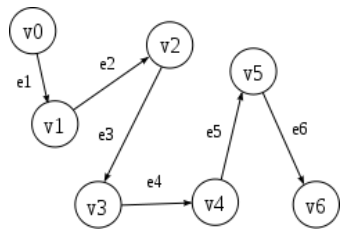
\includegraphics[width=8cm, height=4cm]{graf1} 
		\label{fig:graf1} 
	\end{figure}
	
Graf memiliki banyak jenis, jenis-jenis graf ini didasarkan pada ada tidaknya \textit{loop} pada suatu graf dan sisi pada graf yang mempunyai orientasi arah. Berdasarkan ada tidaknya \textit{loop} pada suatu graf digolongkan menjadi dua jenis :
\begin{enumerate}
	\item Graf Sederhana
	
	Graf ini tidak mempunyai sisi ganda.
	\item Graf tak-sederhana
	
	Graf ini mempunyai sisi ganda.
\end{enumerate}

Berdasarkan orientasi arah pada sisi, secara umum graf dibedakan menjadi 2 jenis :
\begin{enumerate}
	\item Graf tak-berarah
	
	Graf yang sisinya tidak mempunyai arah. Pada graf ini urutan sisi tidak diperhatikan.
	\item Graf berarah
	
	Graf yang sisinya mempunyai arah. Pada graf ini urutan sisi diperhatikan. \cite{referensiCA5}
\end{enumerate}

Sebuah graf dinyatakan sebagai struktur data yang terdiri dari simpul dan sisi yang membangun hubungan antar simpul. Terdapat dua macam representasi graf yaitu \textit{adjacency list} dan \textit{adjacency matrix}. \cite{referensiGraph1}
\subsection{Adjacency List}
Adjacency list merupakan bentuk representasi dari seluruh sisi dalam sebuah graf sebagai suatu senarai (\textit{linked list}). Simpul-simpul yang dihubungkan merupakan simpul-simpul yang saling terkait. Dalam implementasinya, adjacency list menggunakan \textit{hash table} untuk menghubungkan satu simpul dengan simpul lain yang saling terkait. Contoh implementasi adjacency list yaitu sebagai berikut :

 	\begin{figure} [H]
		\centering  
		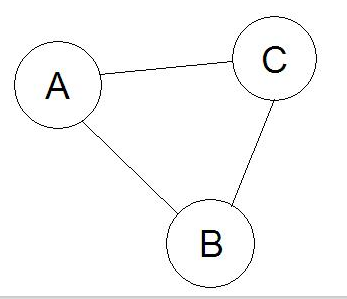
\includegraphics[width=4cm, height=4cm]{adjacencylist} 
		\caption[\textit{Undirected Cyclic Graph}]{\textit{Undirected Cyclic Graph}}
		\label{fig:GambarAL} 
	\end{figure}
	
	Graf pada gambar \ref{fig:GambarAL} dapat direpresentasikan melalui tabel \ref{tabelAL} :
	
	
	\begin{table}[H]
\centering
\caption{Tabel Representasi Adjacency List}
\begin{tabular}{|c|p{2cm}|c|}
\hline
Vertex & Adjacency & Array of Adjacent\\
\hline
a & adjacent to & b,c \\
\hline
b & adjacent to & a,c \\
\hline
c & adjacent to & a,b\\
\hline
\end{tabular}
\label{tabelAL}
\end{table}

\subsection{Adjacency Matrix}
Adjacency Matrix merupakan representasi matrix $N \times N$ yang menyatakan hubungan antar simpul dalam suatu graf. Kolom dan baris menyatakan simpul-simpul, sedangkan nilai entri dari matrix menyatakan hubungan antar simpul. Contoh implementasi adjacency matrix yaitu sebagai berikut :

\begin{figure} [H]
		\centering  
		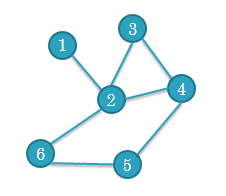
\includegraphics[width=5cm, height=4cm]{adjacencymatrix} 
		\caption[\textit{Undirected Cyclic Graph}]{\textit{Undirected Cyclic Graph}}
		\label{fig:GambarAM} 
	\end{figure}


Graf pada gambar \ref{fig:GambarAM} dapat direpresentasikan melalui tabel \ref{tabelAM} :


\begin{table}[H]
\centering
\caption{Tabel Representasi Adjacency Matrix}
\begin{tabular}{|c|c|c|c|c|c|c|}
\hline
v & 1 & 2 & 3 & 4 & 5 & 6 \\
\hline
1 & 0 & 1 & 0 & 0 & 0 & 0 \\
\hline
2 & 1 & 0 & 1 & 1 & 0 & 1 \\
\hline
3 & 0 & 1 & 0 & 1 & 0 & 0 \\
\hline
4 & 0 & 1 & 1 & 0 & 1 & 0 \\
\hline
5 & 0 & 0 & 0 & 1 & 0 & 1 \\
\hline
6 & 0 & 1 & 0 & 0 & 1 & 0 \\
\hline
\end{tabular}
\label{tabelAM}
\end{table}
